\documentclass{beamer}
\usetheme{UU.SE}

\author{Erik Grafstr\"{o}m \\
        Fartash Nejad \\
        Stephan Brandauer \\
        Jan Daniel Bothma}
\date{September, 20th, 2011}
\institute{Uppsala University\\Department of Information Technology}
\title{Project CS}

\begin{document}

\begin{frame}[plain]
  \titlepage
\end{frame}

\section{Hello!}
\begin{frame}
  \frametitle{Who are We?}
  \begin{itemize}
    \item Stephan Brandauer\\
      {\small Born and raised in Austria, studied in Northern Germany. \\
      Bachelor in Cognitive Informatics}
    \item Jan Daniel Bothma\\
      {\small Born in South Africa, 
      Bachelor in Computer Science from University of Warwick, England}
    \item Erik Grafstr\"{o}m\\
      {\small Born and raised in Sweden, 
      Bachelor in Computer and Information Engineering from Uppsala University}
    \item Fartash Nejad\\
      {\small Born and raised in Iran, 
      Bachelor in Software Engineering}	
  \end{itemize}
\end{frame}

\section{Project CS}

\begin{frame}
  \frametitle{Why are We here?}
  \begin{itemize}
    \item<1-> to tell you about Project CS!
    \item<2-> 30 credit point course, 100\%
    \item<3-> develop software like you would in the real world
    \item<4-> work in a big(!) team in a projectroom
    \item<5-> pick one of two projects
  \end{itemize}
\end{frame}

\begin{frame}
  \frametitle{What is cool about Project CS?}
  \begin{itemize}
    \item<1-> real customer
    \item<2-> very practical
    \item<3-> often a springboard for a Master Thesis or a job
    \item<4-> diversity
  \end{itemize}
\end{frame}

\begin{frame}
  \frametitle{Diversity!}
  \begin{center}
   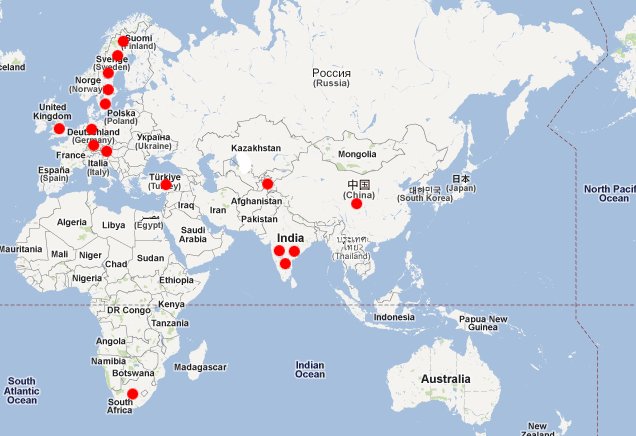
\includegraphics[width=7cm]{images/map.png}
  \end{center}
\end{frame}

\begin{frame}
  \frametitle{What is not so cool about Project CS?}
  \begin{itemize}
    \item big commitment \pause
    \item very practical \pause
    \item a {\bf lot} of work, 8.00 to 17.00, 5 days a week \pause
      \item no results $\rightarrow$ problems with
        \begin{itemize}
          \item the examinator \pause
          \item the customer \pause
          \item your team \pause
        \end{itemize}
  \end{itemize}
\end{frame}

\begin{frame}
  \frametitle{Methodology}
  \begin{itemize}
    \item Erlang
      \begin{itemize}
        \item a functional programming language \pause $\leftarrow$ this is nice \pause
        \item great for writing distributed software \pause
        \item created by Ericsson \pause
        \item parts developed at Polacksbacken (increasing performance) \pause
      \end{itemize}
    \item Agile Software Development (more details later) \pause
    \item Companies behind the projects
    \begin{itemize}
      \item Mobile Arts (Stockholm)
      \item Erlang Solutions (Uppsala/Stockholm)
    \end{itemize}
  \end{itemize}
\end{frame}

\section{Project 1: Mobile Arts GSM Call Service}

\begin{frame}
	\frametitle{Mobile Arts team}
	\begin{center}
		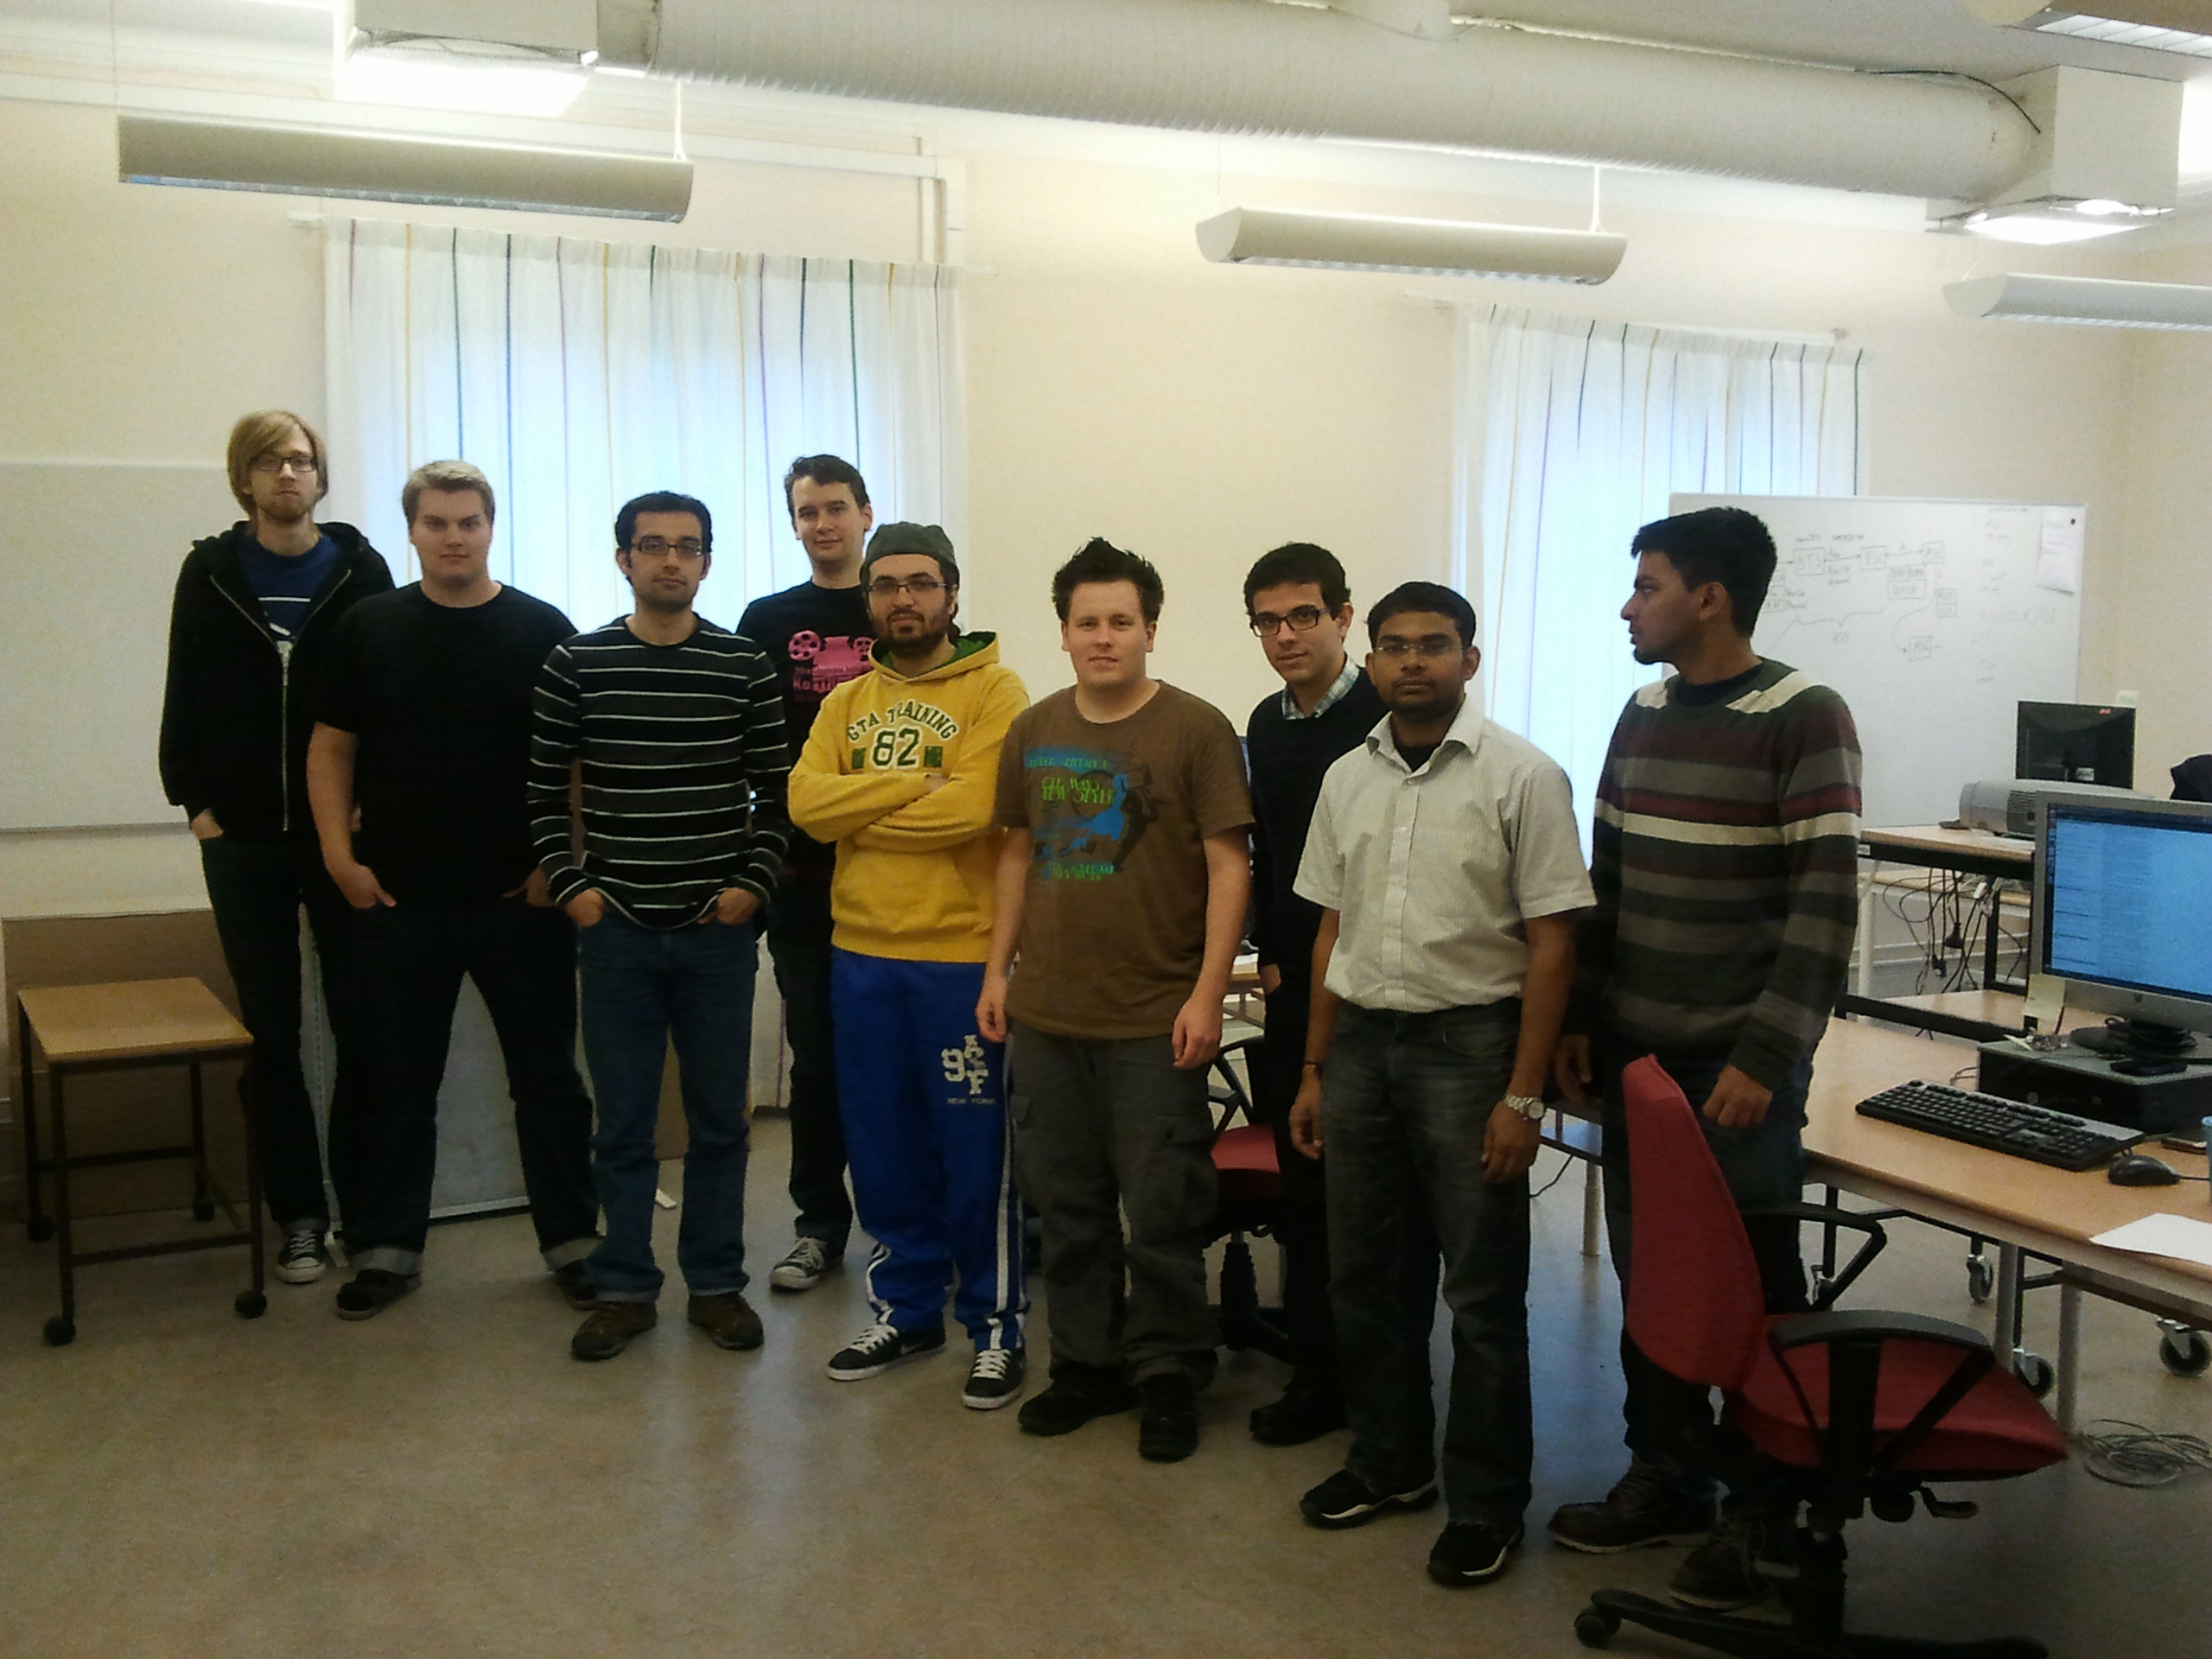
\includegraphics[width=8cm]{images/mobile_arts/team.jpg}
	\end{center}
\end{frame}

\begin{frame}
	\frametitle{Our customer}

 	\begin{center}
		
\includegraphics[width=3cm]{images/mobile_arts/mobilearts_logo.pdf}
	\end{center}	

	\begin{itemize}

	\item
	Mobile Arts provides real-time voice, text messaging and positioning telecom
	products to international GSM/3G/4G operators.

		\begin{itemize}
		\item
		SMS centre
		\item
		Voice mail system
		\item
		GPS positioning system
		\end{itemize}

	\item
	Mobile Arts uses Erlang/OTP as development environment

	\item
	Mobile Arts has taken part in all CS projects since 2005

	\end{itemize}

\end{frame}

\begin{frame}
	\frametitle{GSM System}
	\begin{center}
		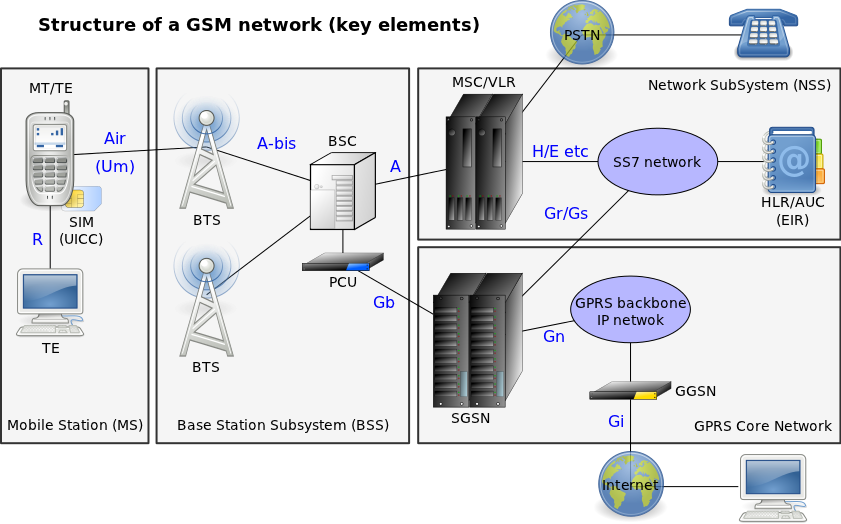
\includegraphics[width=\columnwidth]{images/mobile_arts/gsm.png}
	\end{center}
\end{frame}

\begin{frame}
	\frametitle{Key system characteristics}

	\begin{itemize}
	
	\item
	Large System Architecture

	\item
	Baseline reuse

	\item
	Distributed structure

	\item
	Telecom standards

	\end{itemize}

\end{frame}

\begin{frame}
	\frametitle{GSM call scenario}

 	\begin{center}
		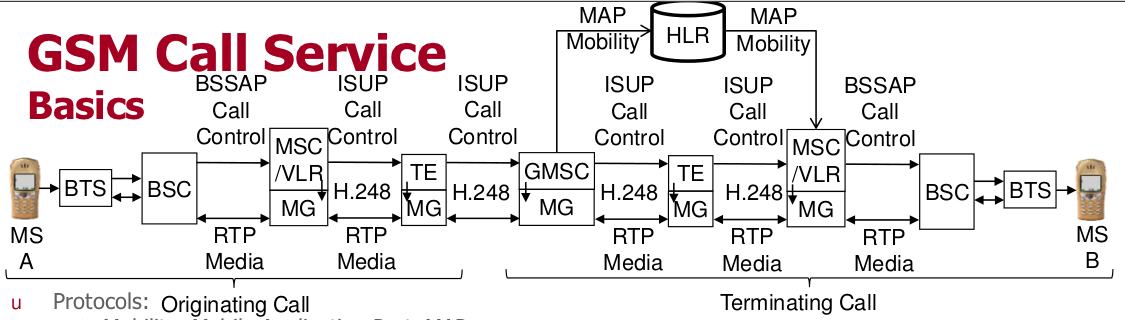
\includegraphics[width=11cm]{images/mobile_arts/gsm_call.png}
	\end{center}

\end{frame}

\begin{frame}
	\frametitle{What we are supposed to do 1/2}

	\begin{itemize}

	\item
	BTS: off-the-shelf nanoBTS
	\item
  	BSC: from Open-BSC project and Mobile Arts thesis projects
   	\item
	(G)MSC/VLR: from CS-10 project (GSM SMS Service)
	\item
	HLR: from Mobile Arts HLR
	\item
	MG and H.248: from CS-09 project (IMS Video Mail Service)

	\end{itemize}

\end{frame}

\begin{frame}
	\frametitle{What we are supposed to do 2/2}

	\begin{itemize}

	\item
	Transit Exchange

	\item
	Connection Service

	\item
	Media Gateway

	\end{itemize}

\end{frame}

\begin{frame}
	\frametitle{How we are supposed to do it}

	\begin{itemize}

	\item
	Agile methods (committing to do stuff, adjusting)

	\item
	Define and divide work

	\item
	Self-organized teams

	\item
	Project room $\rightarrow$ Working agreement

	\item
	FIKA (preferably Kladdkaka)

	\end{itemize}

\end{frame}

\section{Project 2: Diplomacy}

\begin{frame}
  \frametitle{Project 2: Diplomacy}
  \begin{itemize}
    \item implement a board game as online service \pause
    \item setting: Europe at 1900
    \item just before World War 1
    \item players try to conquer the bigger part of europe to win
    \item tactical war game without random elements
  \end{itemize}
\end{frame}

\begin{frame}
  \frametitle{Project 2: Diplomacy}
  \begin{itemize}
    \item players spend a lot of time communicating and making deals \pause
    \item and {\bf breaking} deals! - backstabbing necessary!
    \item can take {\bf very} long (board: 4h-12h)
    \item long history of playing by mail \pause
    \item we have to implement that (play by e-mail)
  \end{itemize}
\end{frame}

\begin{frame}
  \frametitle{The Game}
  \begin{center}
    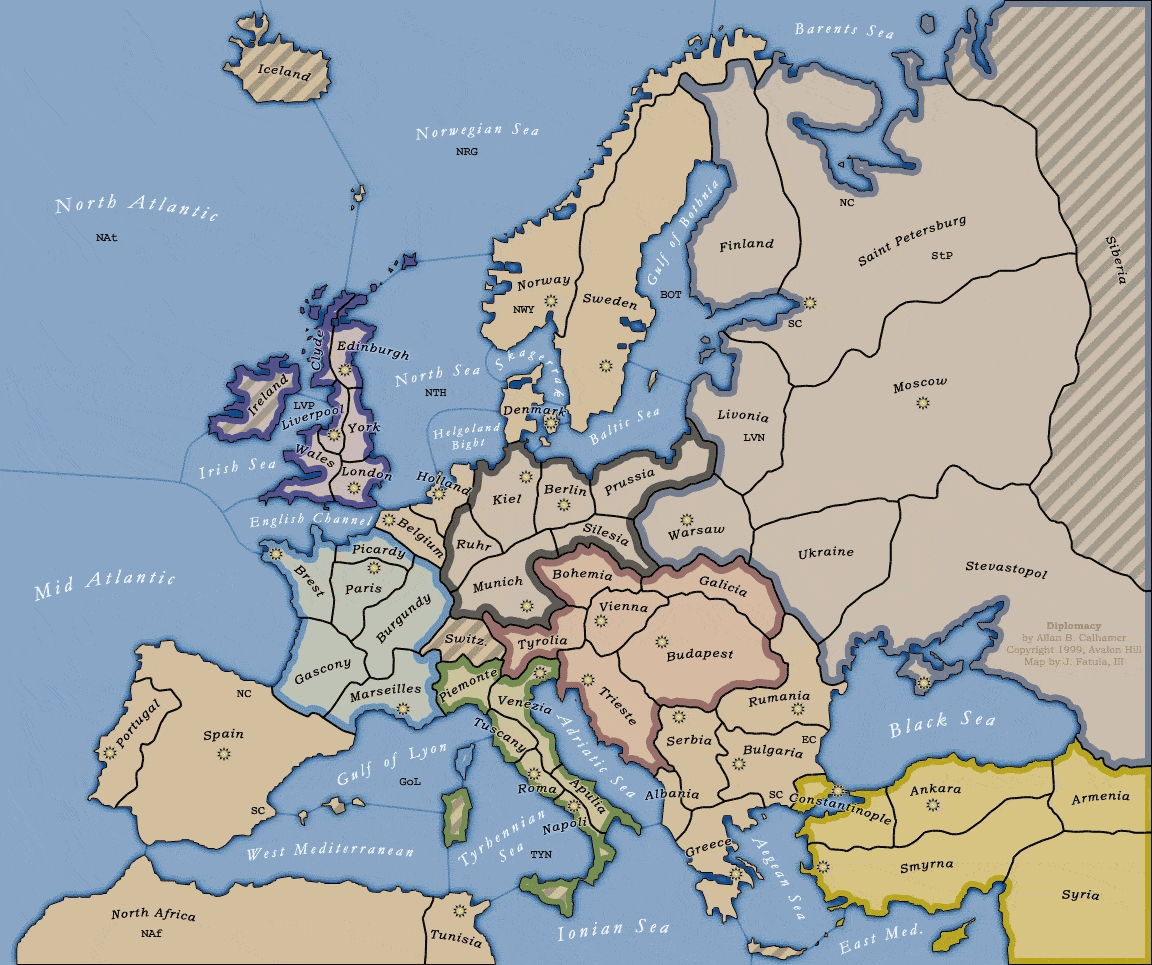
\includegraphics[width=7cm]{images/diplomacy/board.jpg}
  \end{center}
\end{frame}

\begin{frame}
  \frametitle{Why are we making a game?}
  \begin{itemize}
    \item Try lots of important tech
    \item e.g. Websockets, XMPP, different databases
    \item scale without reconfiguration
    \item survive failure
  \end{itemize}
\end{frame}

\begin{frame}
  \frametitle{Our Customer: Erlang Solutions}
  \begin{itemize}
    \item Erlang Consulting (helping solve problems)
    \item "Your scalability architects"
    \item London, Krakow, Stockholm, Uppsala
    \item Founder, Author, Erlang Developer Francesco Cessarini studied here
  \end{itemize}
\end{frame}

\begin{frame}
  \frametitle{Who the Team is}\begin{center}
  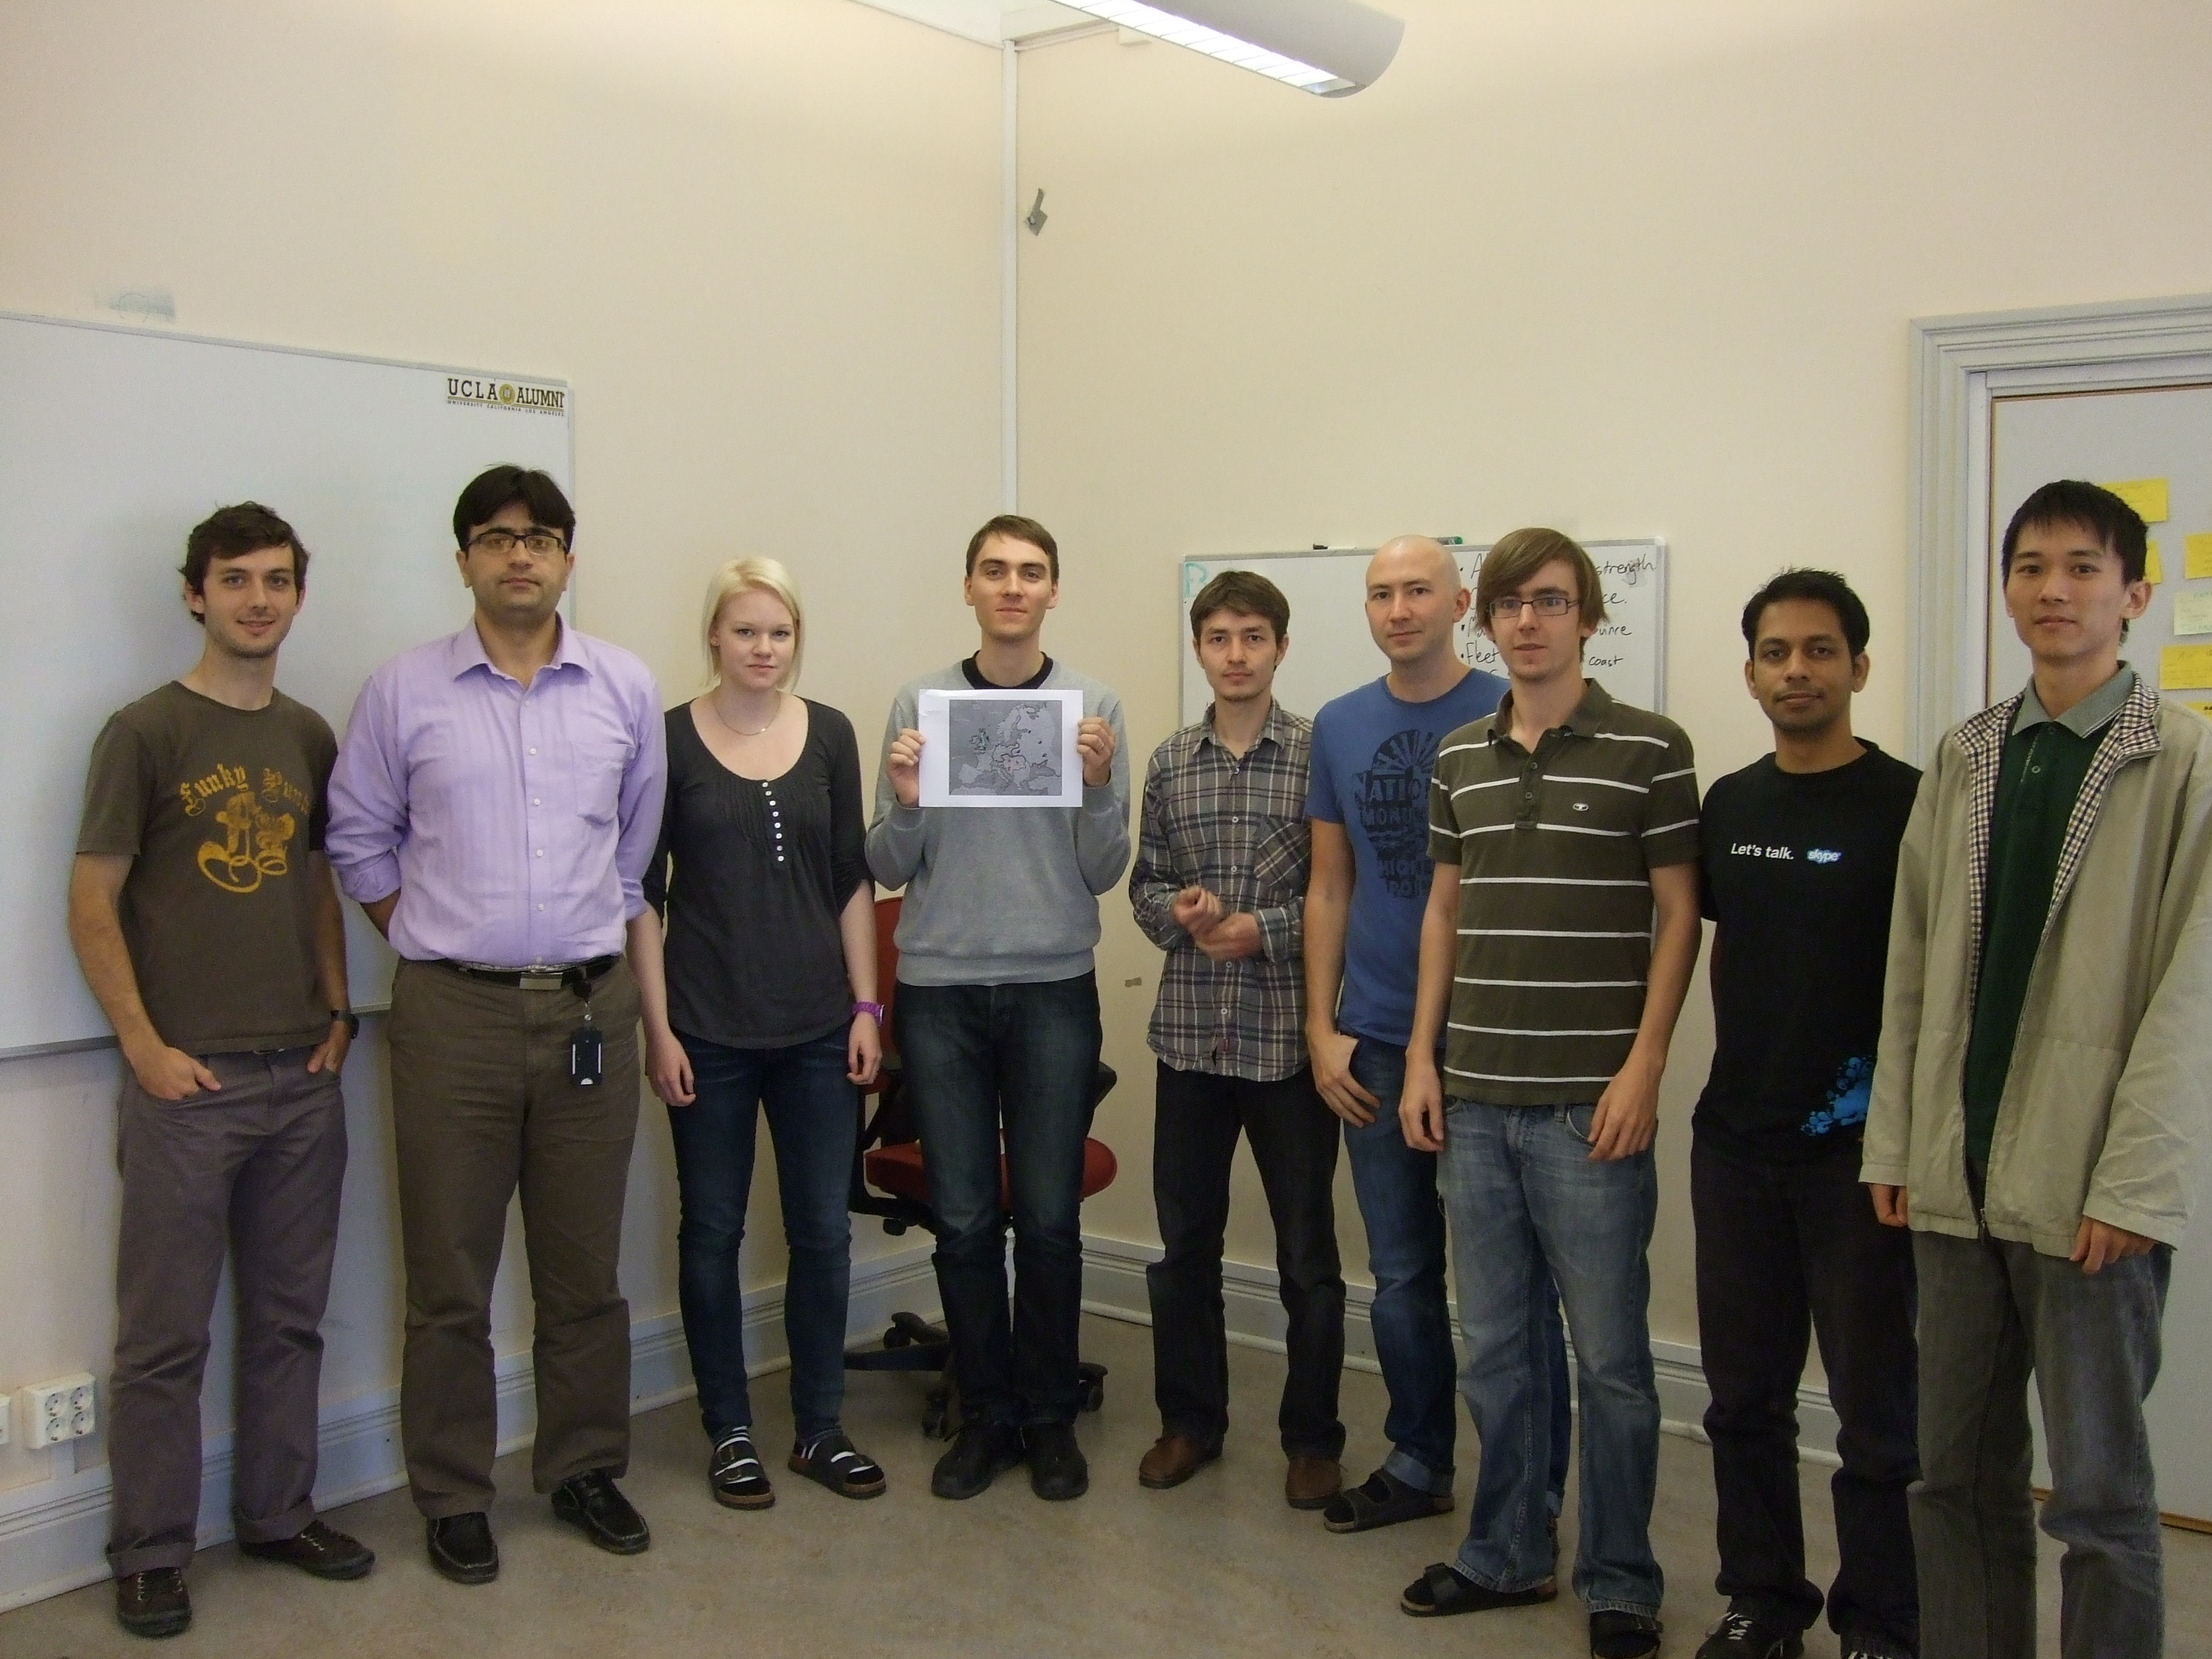
\includegraphics[width=7cm]{images/diplomacy/DSCF6545.jpg}
  \end{center}
\end{frame}

\begin{frame}
  \frametitle{How we are Working}
  \begin{itemize}
   \item SCRUM methodology
   \begin{itemize}
     \item project management system \pause
     \item tells you how to work together \pause
     \item involves lots of sticky notes \pause
     \item working closely with a ``customer'' (erlang solutions) \pause
     \item divide work in small tasks \pause
     \item responsibilities for tasks \pause
     \item It works!
   \end{itemize}
  \end{itemize}

\end{frame}

\begin{frame}
  \frametitle{How we are Working}
  \begin{center}
   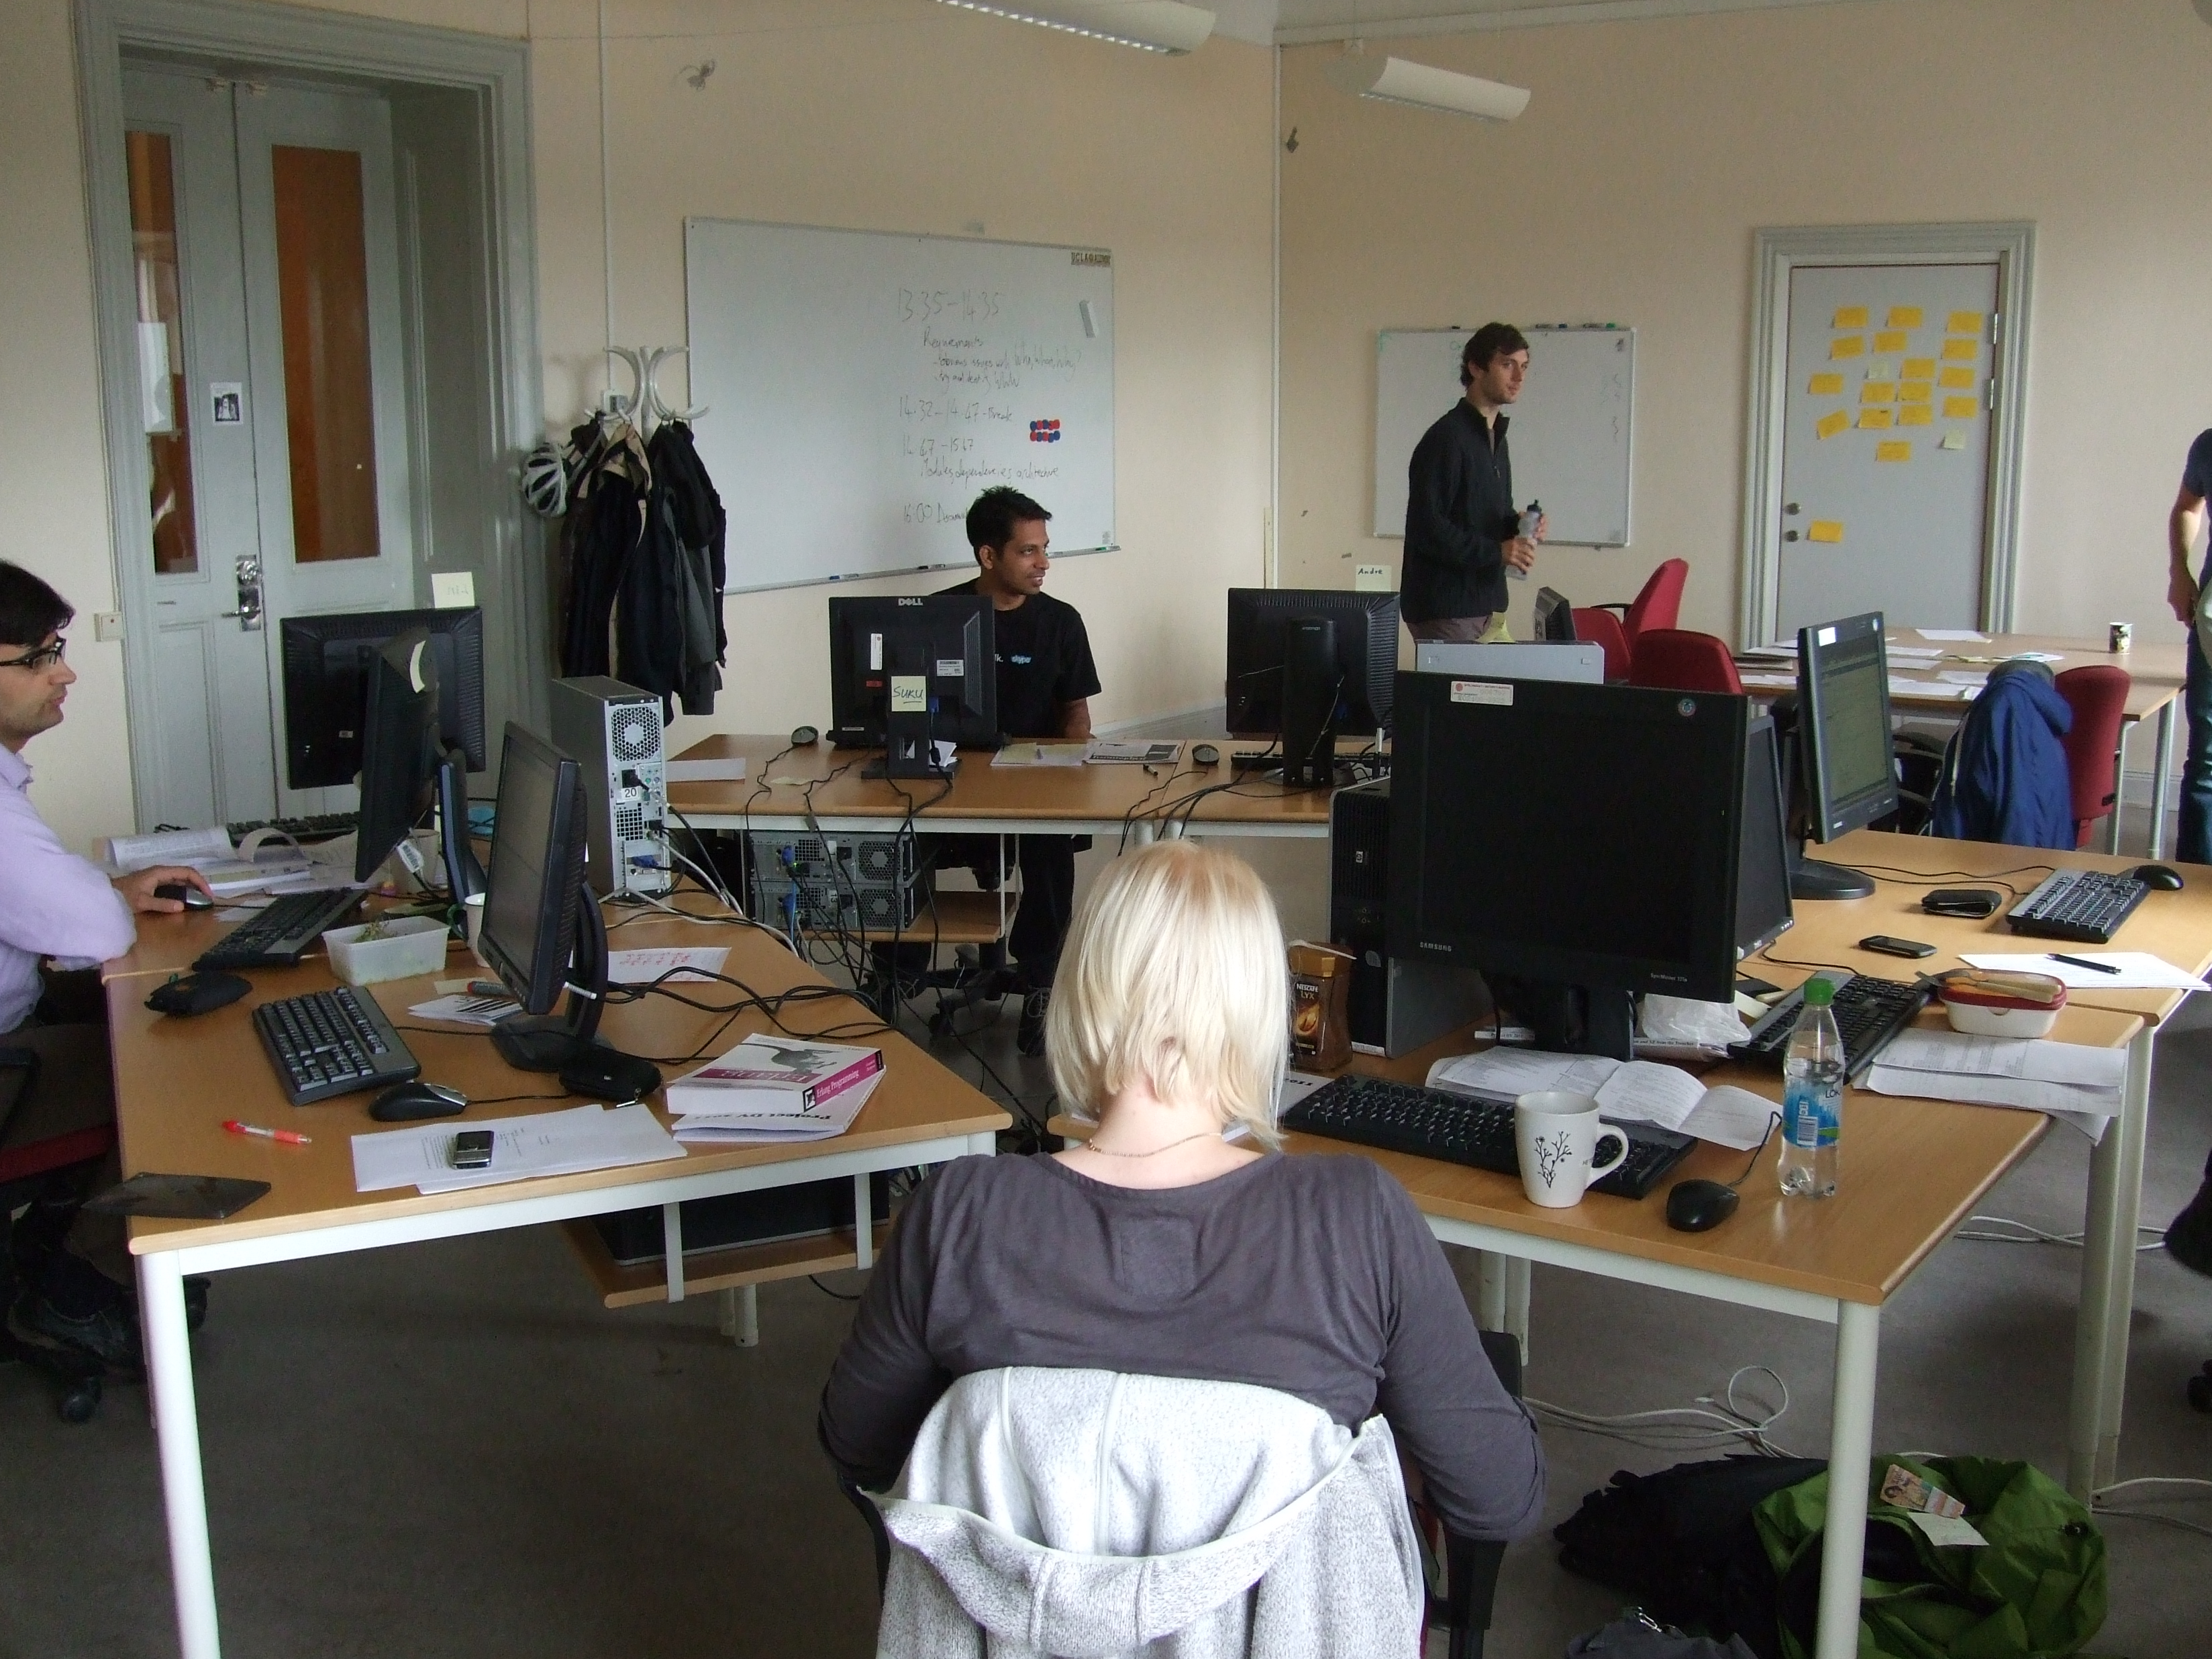
\includegraphics[width=7cm]{images/diplomacy/DSCF6548.jpg}
  \end{center}
\end{frame}

\begin{frame}
  \frametitle{How we are Working}
  \begin{center}
   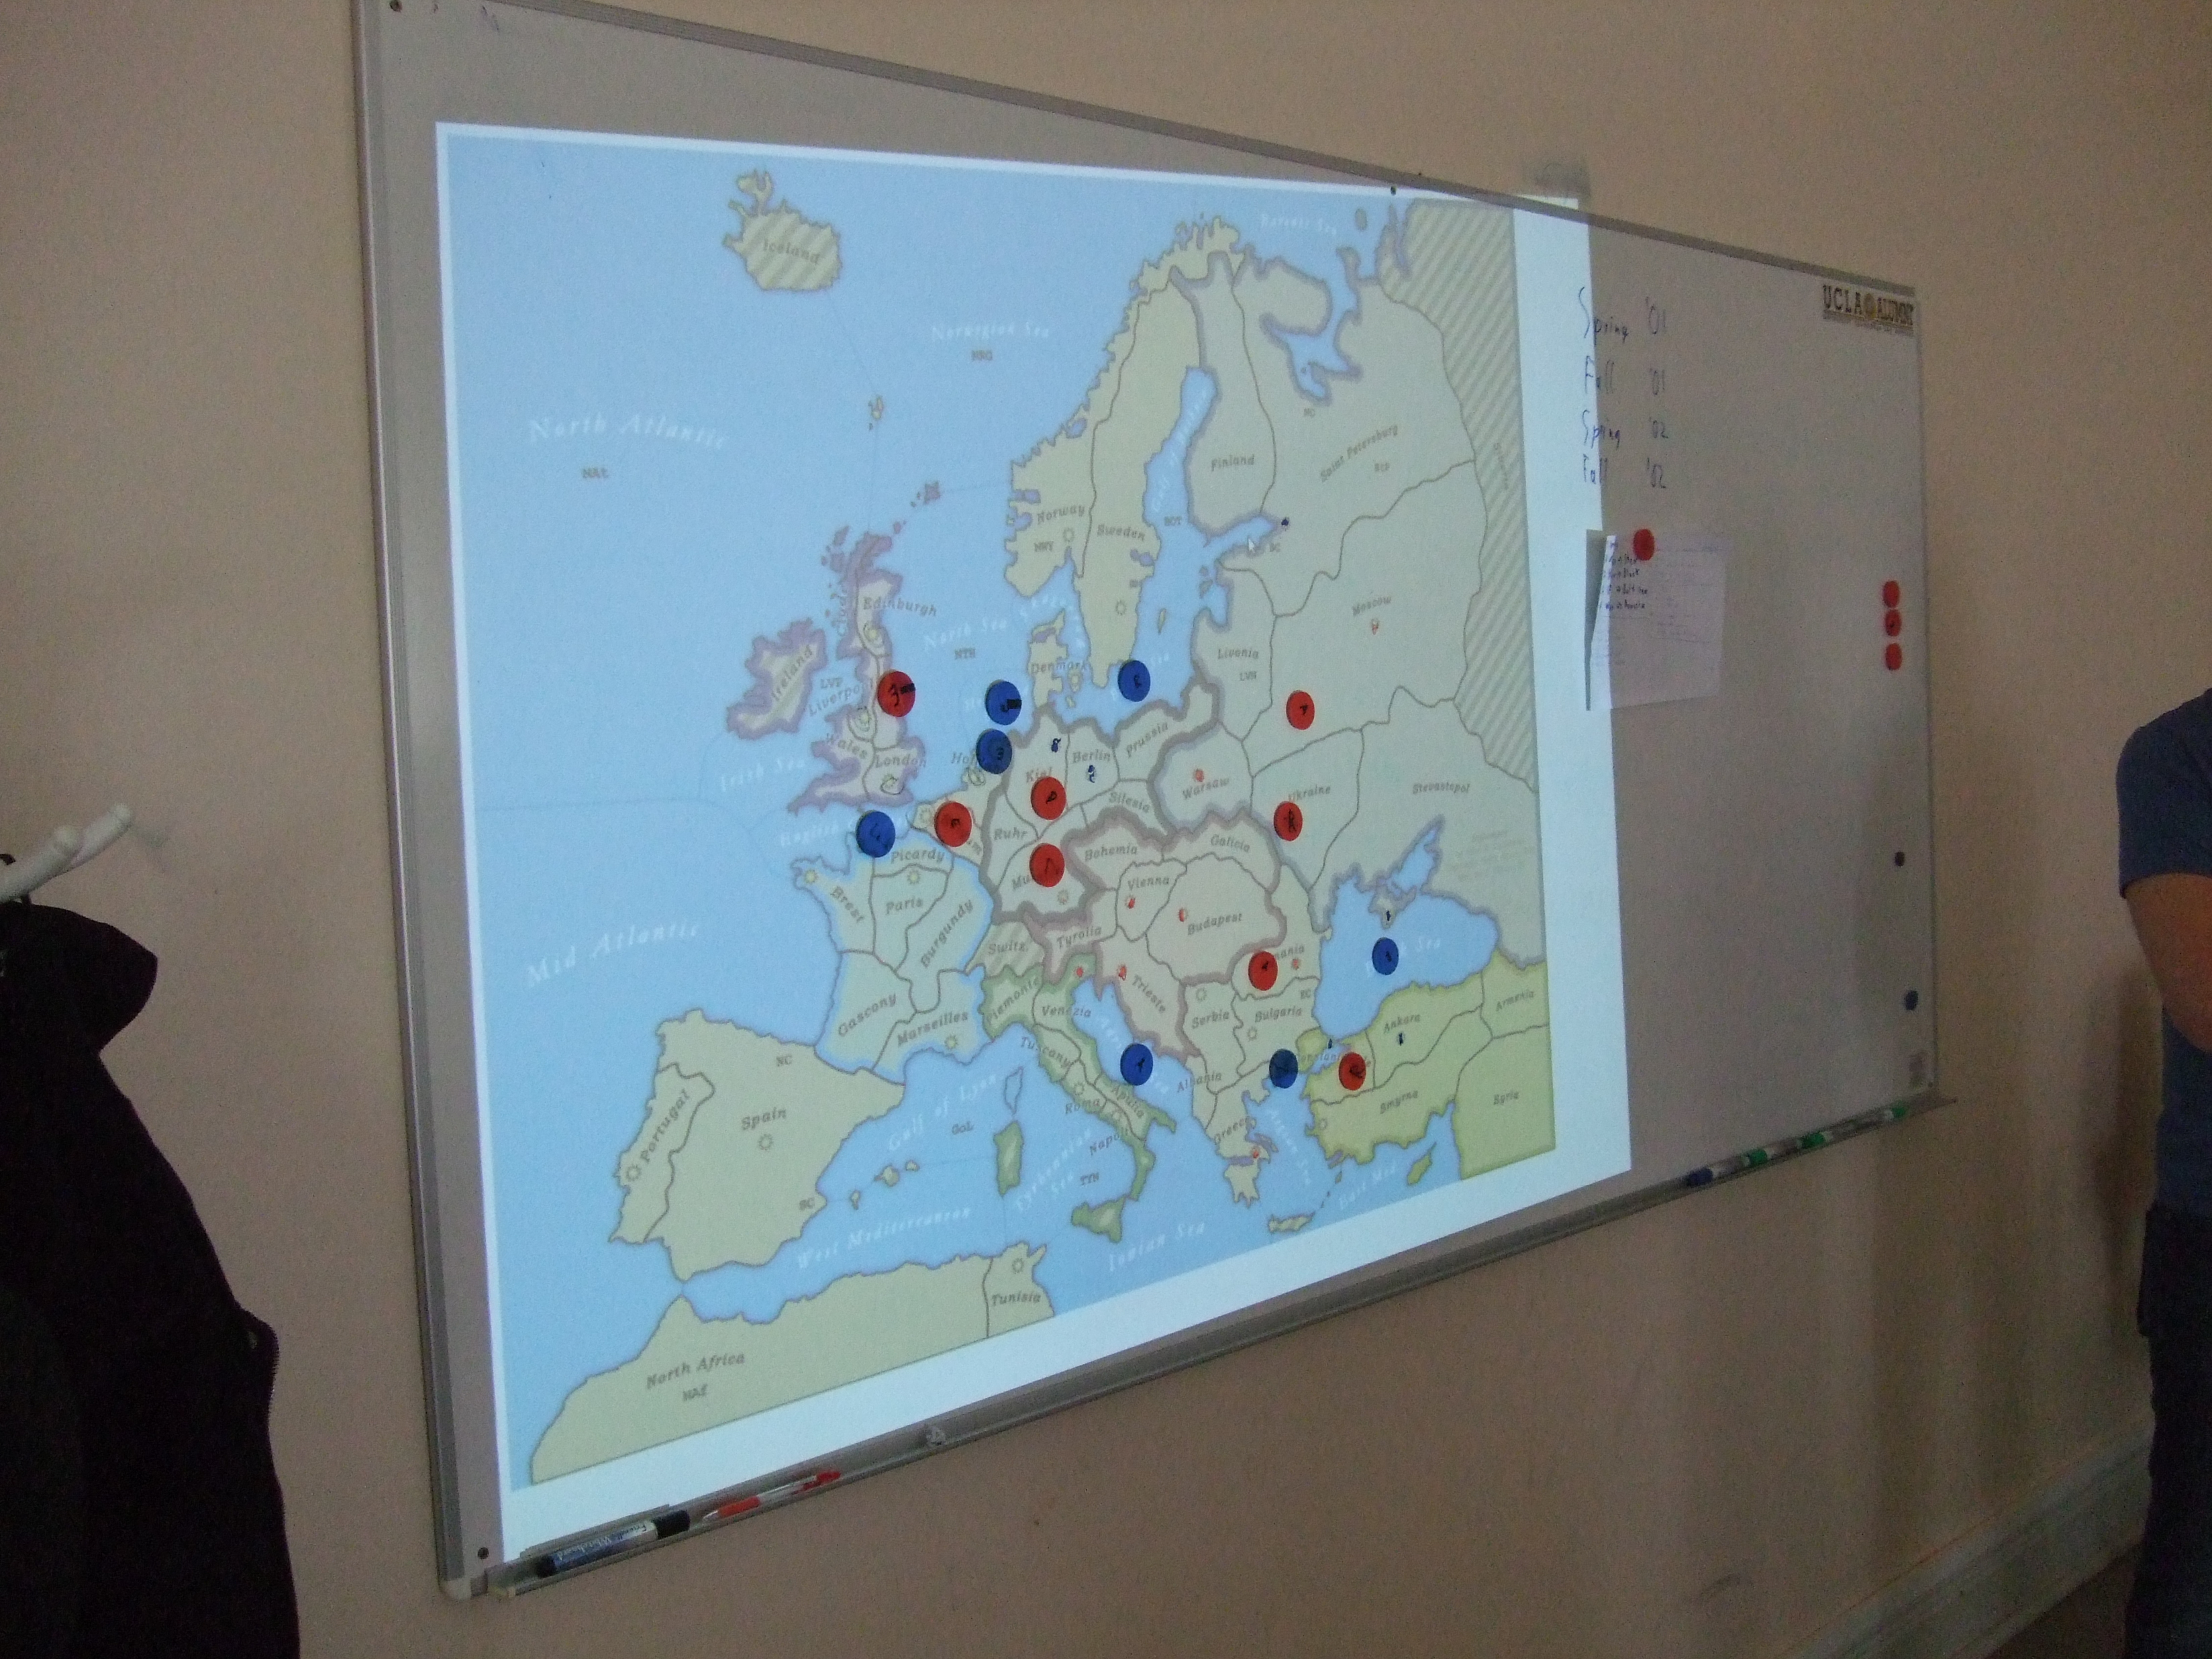
\includegraphics[width=7cm]{images/diplomacy/DSCF6547.jpg}
  \end{center}
\end{frame}

\section{The end}

\begin{frame}
  \frametitle{The last slide}
  \begin{center}
	\huge{Questions?}
  \end{center}
\end{frame}

\end{document}
